\documentclass{beamer}

\usepackage[russian]{babel}
\usepackage[utf8]{inputenc}
\usepackage[outputdir=cache]{minted}

\usetheme{Madrid}
\usecolortheme{dove}
\setbeamertemplate{blocks}[rounded][shadow=false]

\title[]{Приложения комплексных чисел к решению геометрических задач}
\institute[]{ФГБОУ ВО «Вятский государственный университет»}
\date{\today}
\author[ ]{Студент ПМИб-2301-52-00 Ступников Григорий Евгеньевич \and К.ф-м.н Пушкарев Игорь Александрович}

\newcommand\frametitleSpec[1]{%
\frametitle{#1}
\section{#1}%
}


% set captions with numbers
\setbeamertemplate{caption}[numbered]

\begin{document}
\begin{frame}
   \centering
\includegraphics[width=0.4\textwidth]{images/vyatsu_logo.png}\\
   \titlepage
\end{frame}
\begin{frame}
   \frametitle{План доклада}

   \tableofcontents

\end{frame}
\begin{frame}
   \frametitleSpec{Введение}
   Метод комплексных чисел -- это расширение алгебраического метода.
   \begin{enumerate}
      \item Проблема состоит в том, что для данного метода отсутствуют программные материалы для внедрения в среду самостоятельного и школьного обучения.
      \item Целью данной работы является изучение метода комплексных чисел при решении геометрических задач, реализация программной верификации решения выбранных задач. Для достижения цели необходимо выполнить следующие задачи:
            \begin{itemize}
               \item Изучить имеющиеся способы применения алгебры комплексных чисел при решении геометрических задач.
               \item Выбрать задачи, на которых будет рассматриваться практическое применение метода.
               \item Решение задач с применением метода комплексных чисел и без них
               \item Сравнение решений задач.
               \item Реализация программной верификации решения задач с применением метода.
            \end{itemize}
   \end{enumerate}
\end{frame}

\begin{frame}
   \frametitleSpec{Основы метода}
   \begin{columns}
      \begin{column}{0.5\textwidth}
         Комплексное число \(z\) -- число вида $x + iy$, где $x,y \in \mathbf{R}, i = \sqrt{-1},z \in \mathbf{C}, \mathbf{C}$ - поле комплексных чисел. У числа \(z\) можно выделить действительную $x = Re(z)$ и мнимую $y=Im(z)$ части.
      \end{column}
      \begin{column}{0.5\textwidth}
         \begin{figure}
            \centering
            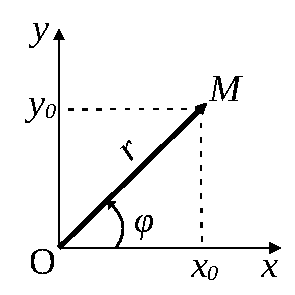
\includegraphics[width=1\textwidth]{images/theory-1.pdf}
            \caption{Изображение числа \(z\) на плоскости}
            \label{img1}
         \end{figure}
      \end{column}
   \end{columns}
\end{frame}

% TASK BEGIN
\begin{frame}
   \frametitleSpec{Задачи}
   \subsection{Задача 1}
   \begin{block}{Задача 1}
      \begin{columns}
         \begin{column}{0.5\textwidth}
            Постановка задачи:
            Точка \(D\) симметрична центру описанной около треугольника ABC окружности, относительно прямой AB.
            Доказать, что расстояние CD выражается формулой
            \begin{equation}
               CD^2 = R^2 +AC^2 + BC^2 - AB^2
               \label{t1:f1}
            \end{equation}
            где R - радиус описанной окружности.
         \end{column}
         \begin{column}{0.5\textwidth}
            \begin{figure}[h]
               \centering
               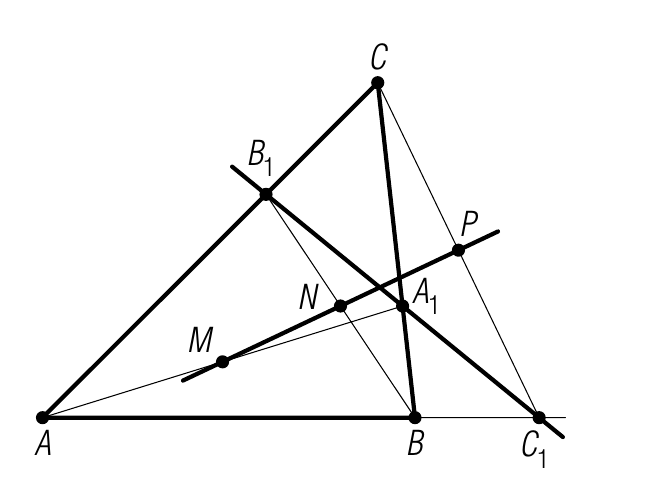
\includegraphics[width=1\textwidth]{images/task1.png}
               \caption{Иллюстрация к задаче}
               \label{t1:im}
            \end{figure}
         \end{column}
      \end{columns}
   \end{block}
\end{frame}

\begin{frame}
   \begin{block}{Задача 1}
      Решение задачи:
      Кратко
   \end{block}
\end{frame}

\begin{frame}
   \begin{block}{Задача 1}
      \begin{block}{Алгоритм программного решения задачи}
         На вход программы передаются координаты свободных точек, в данном примере это координаты точек \(A,B,C,A_1\). По данным входным данным строится прямая, пересекающая стороны \(BC\), \(CA\), \(AB\) треугольника \(ABC\), в точках \(A_1\) , \(B_1\) , \(C_1\).
      \end{block}
   \end{block}
\end{frame}

\begin{frame}
   Демонстрация работы
\end{frame}
% TASK END

% TASK BEGIN
\begin{frame}
   \subsection{Задача 2}
   \begin{block}{Задача 2}
      Постановка задачи:

      Доказать, что если некоторая прямая пересекает прямые, содержащие стороны \(BC\), \(CA\), \(AB\) треугольника \(ABC\), в точках \(A_1\) , \(B_1\) , \(C_1\) соответственно, то середины отрезков \(AA_1\) , \(BB_1\) , \(CC_1\) коллинеарны.

      \begin{figure}[h]
         \centering
         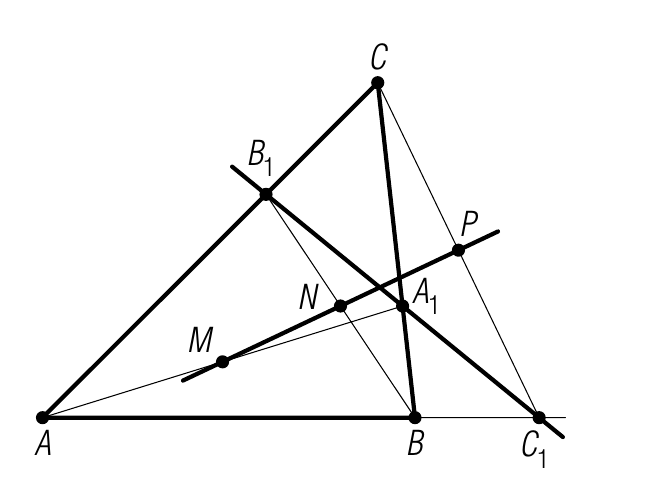
\includegraphics[width=0.4\textwidth]{images/task1.png}
         \label{task2}
      \end{figure}
   \end{block}
\end{frame}

\begin{frame}
   \begin{block}{Задача 2}
      Решение задачи:
      Кратко
   \end{block}
\end{frame}

\begin{frame}
   \begin{block}{Задача 2}
      \begin{block}{Алгоритм программного решения задачи}
         На вход программы передаются координаты свободных точек, в данном примере это координаты точек \(A,B,C,A_1\). По данным входным данным строится прямая, пересекающая стороны \(BC\), \(CA\), \(AB\) треугольника \(ABC\), в точках \(A_1\) , \(B_1\) , \(C_1\).
      \end{block}
   \end{block}
\end{frame}

\begin{frame}
   Демонстрация работы
\end{frame}
% TASK END

% TASK BEGIN
\begin{frame}
   \subsection{Задача 3}
   \begin{block}{Задача 3}
      Постановка задачи:

      Доказать, что если некоторая прямая пересекает прямые, содержащие стороны \(BC\), \(CA\), \(AB\) треугольника \(ABC\), в точках \(A_1\) , \(B_1\) , \(C_1\) соответственно, то середины отрезков \(AA_1\) , \(BB_1\) , \(CC_1\) коллинеарны.

      \begin{figure}[h]
         \centering
         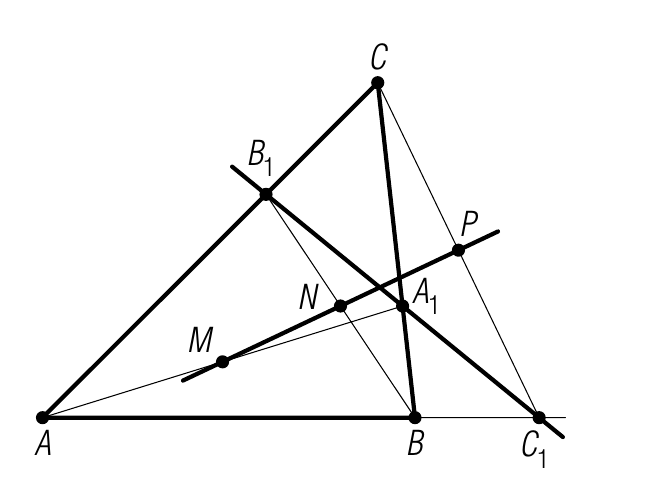
\includegraphics[width=0.4\textwidth]{images/task1.png}
         \label{task3}
      \end{figure}
   \end{block}
\end{frame}

\begin{frame}
   \begin{block}{Задача 3}
      Решение задачи:
      Кратко
   \end{block}
\end{frame}

\begin{frame}
   \begin{block}{Задача 3}
      \begin{block}{Алгоритм программного решения задачи}
         На вход программы передаются координаты свободных точек, в данном примере это координаты точек \(A,B,C,A_1\). По данным входным данным строится прямая, пересекающая стороны \(BC\), \(CA\), \(AB\) треугольника \(ABC\), в точках \(A_1\) , \(B_1\) , \(C_1\).
      \end{block}
   \end{block}
\end{frame}

\begin{frame}
   Демонстрация работы
\end{frame}
% TASK END

% TASK BEGIN
\begin{frame}
   \subsection{Задача 4}
   \begin{block}{Задача 4}
      Постановка задачи:

      Доказать, что если некоторая прямая пересекает прямые, содержащие стороны \(BC\), \(CA\), \(AB\) треугольника \(ABC\), в точках \(A_1\) , \(B_1\) , \(C_1\) соответственно, то середины отрезков \(AA_1\) , \(BB_1\) , \(CC_1\) коллинеарны.

      \begin{figure}[h]
         \centering
         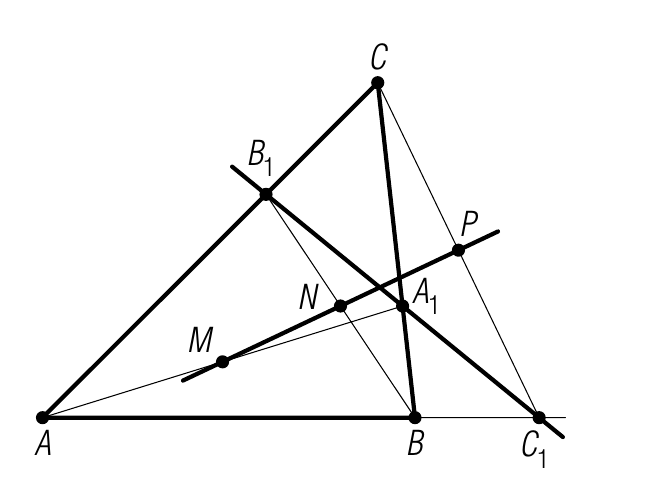
\includegraphics[width=0.4\textwidth]{images/task1.png}
         \label{task4}
      \end{figure}
   \end{block}
\end{frame}

\begin{frame}
   \begin{block}{Задача 4}
      Решение задачи:
      Кратко
   \end{block}
\end{frame}

\begin{frame}
   \begin{block}{Задача 4}
      \begin{block}{Алгоритм программного решения задачи}
         На вход программы передаются координаты свободных точек, в данном примере это координаты точек \(A,B,C,A_1\). По данным входным данным строится прямая, пересекающая стороны \(BC\), \(CA\), \(AB\) треугольника \(ABC\), в точках \(A_1\) , \(B_1\) , \(C_1\).
      \end{block}
   \end{block}
\end{frame}

\begin{frame}
   Демонстрация работы
\end{frame}
% TASK END

% TASK BEGIN
\begin{frame}
   \subsection{Задача 5}
   \begin{block}{Задача 5}
      Постановка задачи:

      Доказать, что если некоторая прямая пересекает прямые, содержащие стороны \(BC\), \(CA\), \(AB\) треугольника \(ABC\), в точках \(A_1\) , \(B_1\) , \(C_1\) соответственно, то середины отрезков \(AA_1\) , \(BB_1\) , \(CC_1\) коллинеарны.

      \begin{figure}[h]
         \centering
         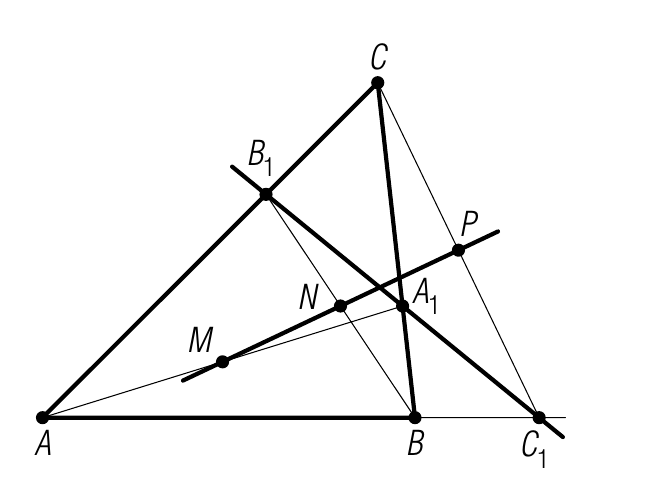
\includegraphics[width=0.4\textwidth]{images/task1.png}
         \label{task5}
      \end{figure}
   \end{block}
\end{frame}

\begin{frame}
   \begin{block}{Задача 5}
      Решение задачи:
      Кратко
   \end{block}
\end{frame}

\begin{frame}
   \begin{block}{Задача 5}
      \begin{block}{Алгоритм программного решения задачи}
         На вход программы передаются координаты свободных точек, в данном примере это координаты точек \(A,B,C,A_1\). По данным входным данным строится прямая, пересекающая стороны \(BC\), \(CA\), \(AB\) треугольника \(ABC\), в точках \(A_1\) , \(B_1\) , \(C_1\).
      \end{block}
   \end{block}
\end{frame}

\begin{frame}
   Демонстрация работы
\end{frame}
% TASK END

% TASK BEGIN
\begin{frame}
   \subsection{Задача 6}
   \begin{block}{Задача 6}
      Постановка задачи:

      Доказать, что если некоторая прямая пересекает прямые, содержащие стороны \(BC\), \(CA\), \(AB\) треугольника \(ABC\), в точках \(A_1\) , \(B_1\) , \(C_1\) соответственно, то середины отрезков \(AA_1\) , \(BB_1\) , \(CC_1\) коллинеарны.

      \begin{figure}[h]
         \centering
         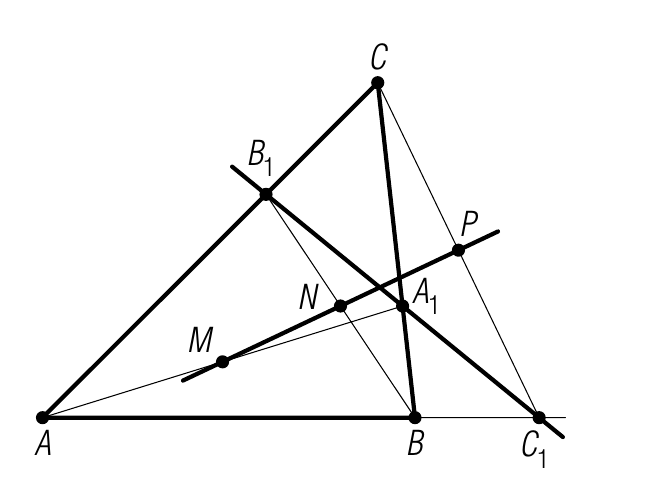
\includegraphics[width=0.4\textwidth]{images/task1.png}
         \label{task6}
      \end{figure}
   \end{block}
\end{frame}

\begin{frame}
   \begin{block}{Задача 6}
      Решение задачи:
      Кратко
   \end{block}
\end{frame}

\begin{frame}
   \begin{block}{Задача 6}
      \begin{block}{Алгоритм программного решения задачи}
         На вход программы передаются координаты свободных точек, в данном примере это координаты точек \(A,B,C,A_1\). По данным входным данным строится прямая, пересекающая стороны \(BC\), \(CA\), \(AB\) треугольника \(ABC\), в точках \(A_1\) , \(B_1\) , \(C_1\).
      \end{block}
   \end{block}
\end{frame}

\begin{frame}
   Демонстрация работы
\end{frame}
% TASK END

\begin{frame}
   \frametitleSpec{О программной реализации задач}
   Решение всех задач написано на языке C++ в виде части программы для решения задач из данной работы.
   Программа (содержащая решение всех задач) поддерживает следующие функции (кроме решения задач):
   \begin{itemize}
      \item запуск нескольких задач из командной строки
      \item вывод информации в виде, пригодном для обработки сторонними программами.
   \end{itemize}
   Кроме того, для тестирования программы написана программа тестирования и тесты к ней.
   \begin{figure}[h]
      \centering
      
\includegraphics[width=0.25\textwidth]{images/cpp-logo.png}
   \end{figure}
\end{frame}
\begin{frame}
   \frametitleSpec{Заключение}

\end{frame}
\begin{frame}
   \begin{center}
      {\huge Спасибо за внимание!}
   \end{center}
\end{frame}
\end{document}
